\hypertarget{praticas-ageis}{%
\section{Comunicação com práticas ágeis}\label{praticas-ageis}}

\hypertarget{comunicacao-com-slack}{%
\subsubsection{\texorpdfstring{Comunicação com \emph{Slack}}{Comunicação com Slack}}\label{comunicacao-com-slack}}

Desde o início da utilização da ferramenta \emph{Slack} a cerca de 20 meses, foram enviadas mais de 26 mil mensagens entre 28 membros. 62\% destas mensagens foram individuais, 32\% foram nos 14 canais públicos disponíveis, e 6\% em canais privados. É válido mencionar também que deste total, aproximadamente um terço foram mensagens de notificação emitidas por \emph{bots}.

Fazendo uma avaliação destes números, é possível observar o uso diário da ferramenta, o que proporcionou uma melhoria significativa na comunicação interna do grupo, principalmente para a colaboração remota dos alunos que estão localizados fora do \emph{CERN}. Algo interessante a melhorar no futuro seria a implementação de filtros mais eficientes a fim de reduzir o número de mensagens enviadas por \emph{bots}. Atualmente o número de mensagens deste tipo é considerável e pode ser parcialmente irrelevante para a maior parte dos desenvolvedores.

\hypertarget{revisao-com-merge-requests}{%
\subsubsection{\texorpdfstring{Revisão com \emph{Merge Requests}}{Revisão com Merge Requests}}\label{revisao-com-merge-requests}}

A adoção da prática de \emph{merge requests} foi uma das contribuições mais notórias em relação a melhorias ágeis. Tendo sido iniciada há aproximadamente dois anos atrás, atualmente mais de 1800 \emph{merge requests} foram realizados entre os 23 repositórios do grupo. Deste número, 95\% dos pedidos passaram por aprovações e foram acrescentados à base de código. No total mais de 2000 discussões ocorreram nesses pedidos, contribuindo na aproximação entre os desenvolvedores na forma de se escrever código. As discussões sobre boas práticas cresceram substancialmente no grupo com o início dos \emph{merge requests}. Ao mesmo tempo facilitou o compartilhamento de soluções já desenvolvidas para um problema identificado durante a revisão. Como uma possível melhoria no futuro, seria interessante o autor do código proporcionar mais informações ao revisor sobre a motivação e comportamento esperado do código a ser revisado, para facilitar sua análise integral pelos revisores.

\hypertarget{documentacao-com-confluence}{%
\subsubsection{\texorpdfstring{Documentação com \emph{Confluence}}{Documentação com Confluence}}\label{documentacao-com-confluence}}

Começando a ser utilizado há 10 meses, a documentação contida no software \emph{Confluence} contém atualmente mais de 250 documentos em uma colaboração de mais de 30 membros e com um total de mais de 4200 acessos. Nos últimos 3 meses a plataforma chegou a possuir quase 500 acessos em uma semana, e documentos contendo apresentações e tutoriais foram os mais visualizados. Na figura \ref{fig:space-analytics} é possível analisar alguns números. Durante o mês de agosto o \emph{Confluence} possuiu quase 1,5 mil acessos, com a página principal possuindo 475 visualizações.

\begin{figure}[H]
    \centering
    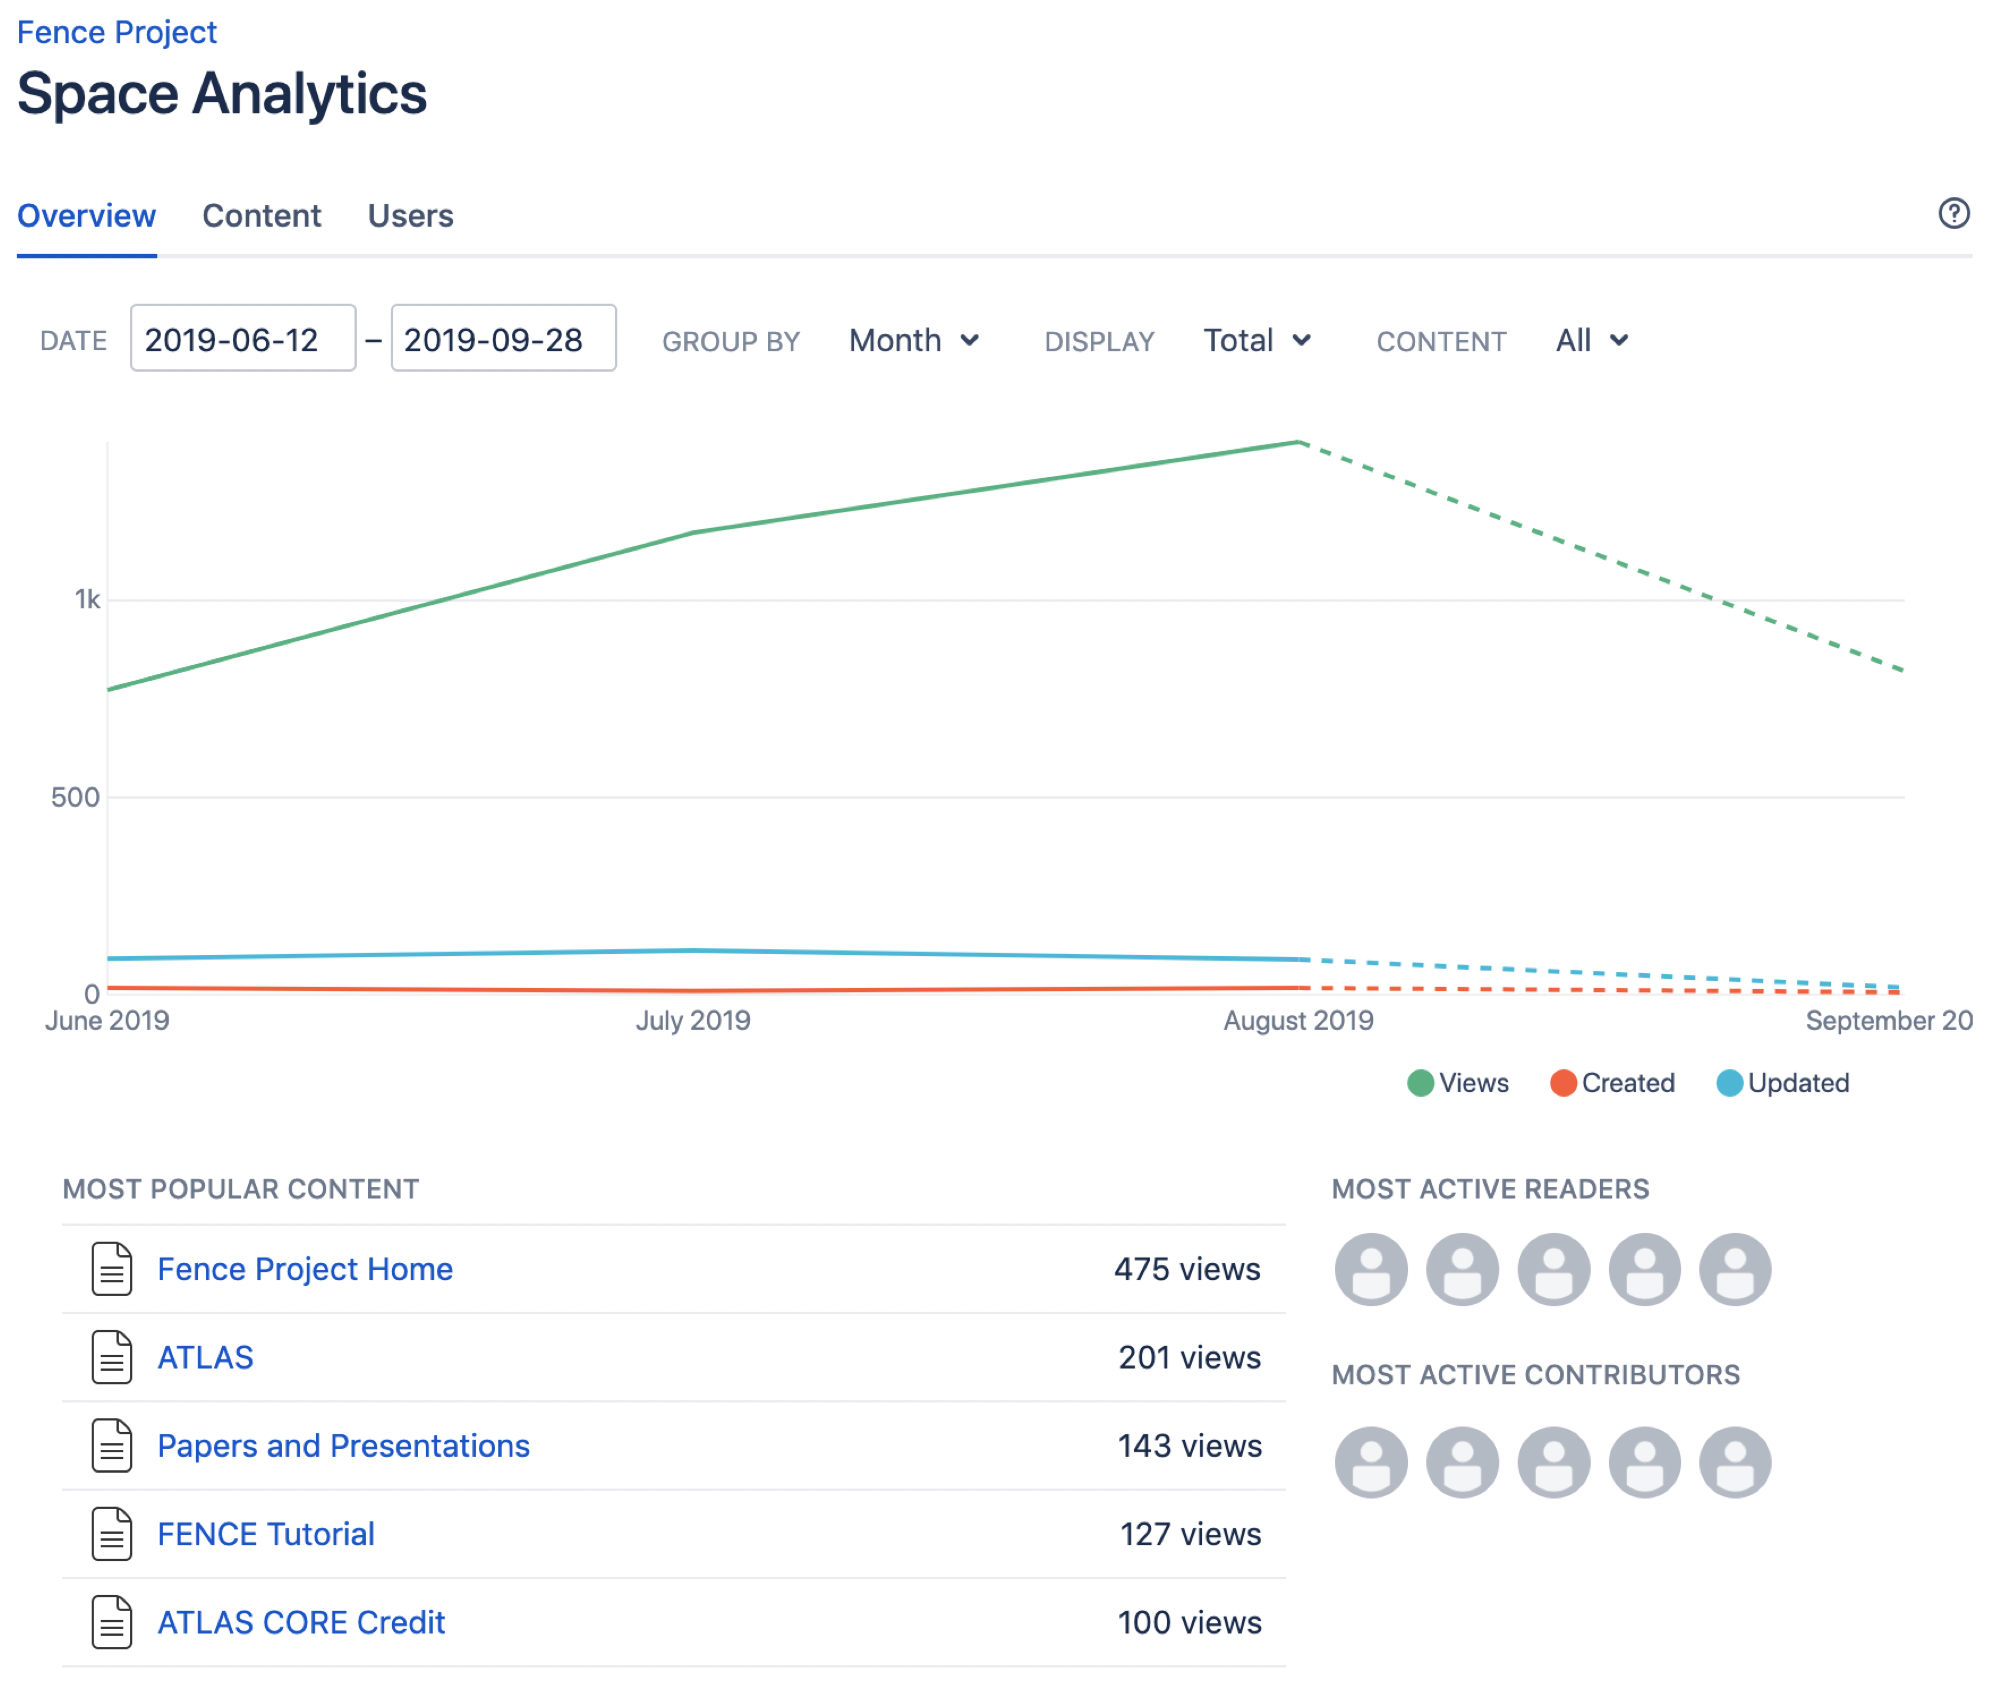
\includegraphics[width=15cm]{source/5-resultados/images/space-analytics-censored.png}
    \caption{Análise de acessos à plataforma \emph{Confluence} do grupo.}
    \label{fig:space-analytics}
\end{figure}

O principal benefício trazido pela plataforma foi a centralização da documentação que anteriormente se encontrava espalhada entre outras ferramentas. Apesar de possuir grande integração nativa com a plataforma \emph{JIRA}, há o desejo futuro em ter mais controle com esta integração, como a adoção do \emph{plugin} \emph{ScriptRunner} que permite uma flexibilização maior, a nível de código, na manipulação de dados entre as duas plataformas.

\hypertarget{validacao-com-linters}{%
\subsubsection{\texorpdfstring{Validações com \emph{Linters}}{Validações com Linters}}\label{validacao-com-linters}}

Começando a ser usado há cerca de um ano, a análise do uso de \emph{linters} é mais subjetiva em relação a resultados. Conversando com os desenvolvedores do grupo, para um programador iniciante os avisos de \emph{linters} podem ocorrer em até 50\% de suas linhas escritas, enquanto para os mais experientes esta ocorrência diminui para uma taxa média de 10\%. De toda forma, seu uso se mostra fundamental por todos, apesar de houver constantes dificuldades em manter todos os \emph{linters} funcionais. Estas dificuldades ocorrem principalmente por conta dos diferentes editores de texto usado pelos desenvolvedores, assim como suas diferentes versões, configurações e condições operacionais.

\hypertarget{plano-de-testes-com-lean-testing}{%
\subsubsection{\texorpdfstring{Plano de testes com \emph{Lean Testing}}{Plano de testes com Lean Testing}}\label{plano-de-testes-com-lean-testing}}

O uso da ferramenta \emph{Lean Testing} se faz presente a pelo menos dois anos. Planos de testes para 6 sistemas foram desenvolvidos desde então, totalizando mais de 1500 \emph{test cases}. Diversas validações foram realizadas a partir destes planos, feitas principalmente por alunos ingressantes.

A utilização desta ferramenta ainda é parcial pelo grupo. Apesar de seus benefícios, para alguns membros há ainda a preferência pelo software \emph{Google Sheets}. O \emph{Lean Testing} estabelece critérios bem definidos sobre como realizar o plano de testes, na tentativa de orientar o desenvolvedor de testes e o testador. Já o \emph{Google Sheets}, como se trata de uma ferramenta genérica para edição de planilhas, possui suporte a mais customizações, como \emph{macros} e \emph{scripts}, mas ao mesmo tempo possui menos funcionalidades específicas de testes, como histórico de execuções.

É notável também a redução recente da atualização dos planos de testes, motivado principalmente por dificuldade de alocação de tempo nesta tarefa durante o processo de trabalho. Para um trabalho futuro há o interesse em revisitar esta questão, na tentativa de compreender como esta atividade pode ser otimizada.

\begin{figure}[H]
    \centering
    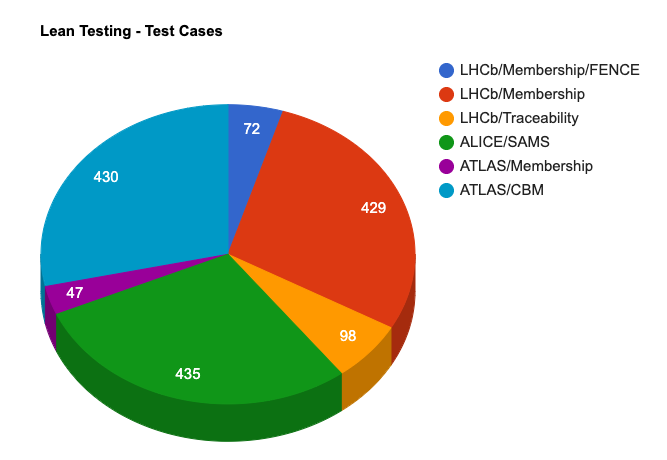
\includegraphics[width=11cm]{source/5-resultados/images/lean-testing.png}
    \caption{Divisão de \emph{test cases} entre os sistemas utilizando o \emph{Lean Testing}.}
    \label{fig:lean-testing}
\end{figure}
